\documentclass[10pt,a4paper]{article}
\usepackage[utf8]{inputenc}
\usepackage[T1]{fontenc}
\usepackage{lmodern}
\input{glyphtounicode}
\pdfgentounicode=1
\usepackage[slovene]{babel}
\usepackage[margin=1.5cm]{geometry}
\usepackage{graphicx,booktabs,hyperref,array}
\hypersetup{colorlinks=true,urlcolor=blue}
\setlength{\parindent}{0pt}
\setlength{\emergencystretch}{2em}
\setlength{\parskip}{4pt}
\renewcommand{\arraystretch}{1.16}
\begin{document}
\begin{center}{\LARGE THUD: opis slike in stabilnost objektov}\\[5pt]
{\large Vmesno poročilo za predstavitev 21. 10. 2026}\\[4pt]
\textbf{Osnutek za poznejši ročni pregled in dopolnitev}\end{center}
\section*{Cilj in postopek}
Robot za dolgoročno karto potrebuje opis vidnih objektov in njihovih odnosov ter ločeno presojo, ali se lahko položaj spremeni med obiski. Trenutna negibnost na fotografiji ni dokaz trajnosti.
\begin{center}\fbox{izbor slik $\rightarrow$ opis/detekcija $\rightarrow$ besedilna presoja $\rightarrow$ vrednotenje $\rightarrow$ poročilo}\end{center}
Prvi korak uporablja sliko, drugi samo zamrznjeni JSON opis. Razredi so \texttt{fixed}, \texttt{movable}, \texttt{uncertain}; izhod vsebuje kratko besedno utemeljitev, ne skritega notranjega razmišljanja.
\section*{Podatki in dve ločeni nalogi}
\begin{center}\small\begin{tabular}{lrr}\toprule
Nabor & Slike & Regije \\ \midrule
Trgovina (dense) & 50 & 678 \\
agtea & 50 & 1021 \\
\bottomrule\end{tabular}\end{center}

Poti, mere in SHA256 vseh slik so preverjeni. To so povezani pogledi istih prostorov, ne 100 neodvisnih prizorov. Oznake vsebujejo vrste in okvirje, ne razredov stabilnosti. \texttt{Products} je lahko skupina; ID velja samo znotraj slike.
\begin{itemize}\item \textbf{Samostojno zaznavanje (discovery):} ločen manifest vsebuje le nevtralni ID slike, slikovno pot, mere in SHA256. Model ne prejme referenčnih imen, regijskih ID, okvirjev ali anotacijskih poti.
\item \textbf{Opisovanje danih regij (supplied):} model prejme anotirane regije, vrne njihove iste ID in imena. Kopirano ime ni detekcijski zadetek.\end{itemize}
\section*{Modeli in nastavitve}
\begin{center}\small\begin{tabular}{lllr}\toprule
Točen model & Uteži & Projektor & VRAM [GiB] \\ \midrule
qwen3.5:4b-bf16 & BF16 & F16 & 8.8 \\
qwen3.5:4b-q4\_K\_M & Q4\_K\_M & BF16 & 3.4 \\
gemma3:4b-it-q4\_K\_M & Q4\_K\_M & ni poročano & 2.8 \\
\bottomrule\end{tabular}\end{center}

Točni tagi: \texttt{qwen3.5:4b-bf16}, \texttt{qwen3.5:4b-q4\_K\_M}, \texttt{gemma3:4b-it-q4\_K\_M}. Tagi in slikovna podpora so preverjeni v uradnem katalogu ter z \texttt{/api/show}. Tudi Qwen slikovna projektorja imata različni natančnosti (F16/BF16). BF16 metapodatki navajajo 33 blokov in nextn\_predict\_layers=1, Q4 pa 32 blokov. Zato to ni strogo izoliran poseg samo v natančnost istih pretvorjenih uteži; vpliv dodatne napovedne plasti ni posebej preverjen. Družin pri različnih natančnostih ne primerjamo kot čiste arhitekturne razlike.
VRAM je največja dodelitev modelu v shranjenih merjenih odgovorih API, ne celotna zasedenost kartice. Projektor: GGUF file type iz metapodatkov, F16=1 in BF16=32. Osnova: podroben prompt brez vsebinskih primerov, $T=0$, seed 42, kontekst 16384, izhod do 8192 tokenov, top-p 0.8, top-k 20, presence penalty 1.5. Enaki izvorni bajti slike; notranje predprocesiranje modelov se lahko razlikuje.

\newpage
\section*{Dejanski obseg in hitrost}Osnovna primerjava: 600/600 merjenih odgovorov, 576 odgovorov ustreza shemi, 24 napak; skladen zapis JSON ima 600 odgovorov. Dodatni prvi korak: 80/80; drugi korak: 120/120. Dodatna Q4 ponovitev: 20/20. Ogrevalni klici so shranjeni ločeno in izključeni iz teh imenovalcev.
\begin{center}\small\begin{tabular}{lllrrrrrr}\toprule
Nabor & Način & Model & OK/vsi & Med. & p90 & Povp. & Izh. tok. & tok/s \\ \midrule
trgovina & samost. & qwen35-bf16 & 50/50 & 8.4 & 17.3 & 10.0 & 486 & 49.9 \\
trgovina & samost. & qwen35-q4 & 50/50 & 2.5 & 5.1 & 3.2 & 477 & 163.1 \\
trgovina & samost. & gemma3-q4 & 50/50 & 3.0 & 5.6 & 3.6 & 545 & 170.0 \\
trgovina & regije & qwen35-bf16 & 49/50 & 9.1 & 13.1 & 9.5 & 1057 & 115.8 \\
trgovina & regije & qwen35-q4 & 50/50 & 5.3 & 8.4 & 5.9 & 1044 & 186.9 \\
trgovina & regije & gemma3-q4 & 46/50 & 6.6 & 9.5 & 6.9 & 1137 & 180.5 \\
agtea & samost. & qwen35-bf16 & 50/50 & 4.2 & 5.7 & 4.4 & 534 & 127.8 \\
agtea & samost. & qwen35-q4 & 50/50 & 2.8 & 4.4 & 3.1 & 564 & 198.9 \\
agtea & samost. & gemma3-q4 & 50/50 & 3.3 & 6.4 & 3.9 & 642 & 182.7 \\
agtea & regije & qwen35-bf16 & 45/50 & 19.1 & 47.5 & 23.5 & 1479 & 64.3 \\
agtea & regije & qwen35-q4 & 47/50 & 7.2 & 10.8 & 7.8 & 1464 & 197.7 \\
agtea & regije & gemma3-q4 & 39/50 & 8.8 & 11.7 & 8.8 & 1487 & 180.5 \\
\bottomrule\end{tabular}\end{center}

\begin{center}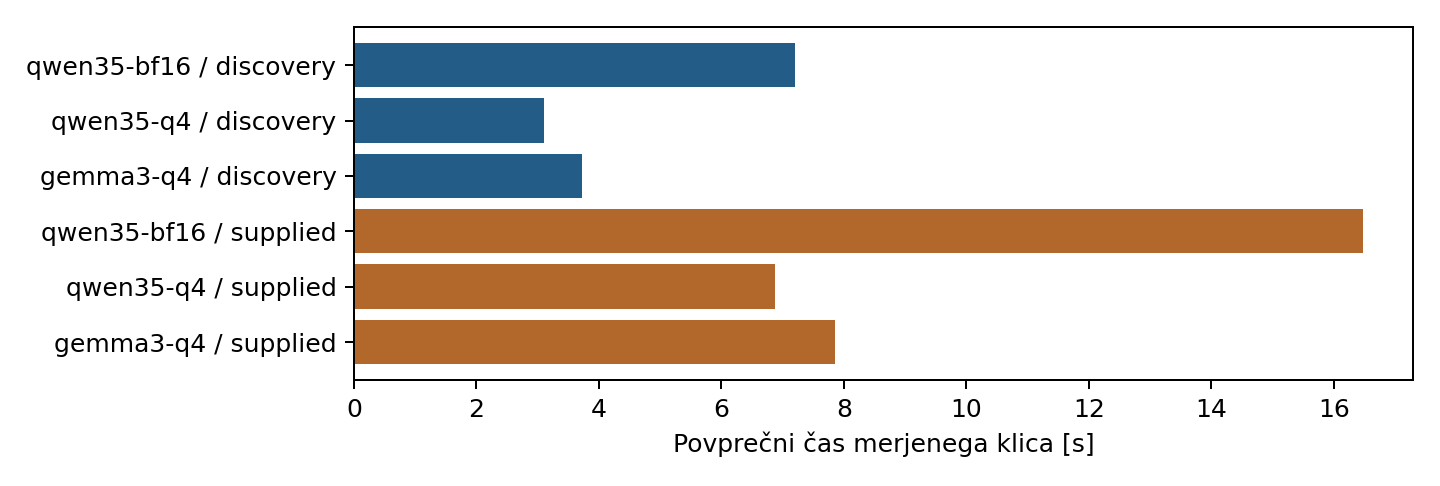
\includegraphics[width=.94\linewidth]{figures/latency.png}\end{center}
Izh. tok. je povprečno število izhodnih tokenov. Časi so sekunde na sliko/klic; p90 uporablja linearno interpolacijo. Čas vključuje vse odgovore z izmerjenim časom, tudi zavrnjeni JSON. Napake prenosa lahko nimajo časa; število takih klicev je v agregatih. Tok/s je vsota izhodnih tokenov deljena z vsoto API časa generiranja. Nalaganje in tokeni so ločeno ohranjeni; end-to-end čas je čas celotne skupine, vključno z ogrevanjem, preverjanjem in zapisovanjem.
Osnovni del: skupni end-to-end čas 77.4 min; ogrevalni klici 114.5 s, od tega API nalaganje 33.3 s; API nalaganje v merjenih klicih 5.7 s. Nalaganje je podmnožica časa zahteve, zato teh časov ne seštevamo.
Pilot: 24 merjenih klicev; linearna ocena osnovnega dela pred polnim zagonom je bila 2.5 h. Ocena ni meritev celotnega izvajanja.

RTX 5090 (32607 MiB), Docker Compose in projektna Ollama. Začetni stari kontejner je izgubil GPU: CPU diagnostika je ohranjena ločeno, kontejner je bil ponovno ustvarjen z GPU override. Veljavni klici preverijo VRAM; delni CPU offload se zavrne. Drug uporabnikov proces je hkrati obremenjeval GPU; ni bil ustavljen. To omejuje primerjavo hitrosti. Različno dolgi odgovori in API predpomnilnik predpon/slikovnega kodiranja dodatno vplivajo na čase; svež HTTP klic ne zagotavlja hladnega predpomnilnika.

\newpage
\section*{Vpliv prompta, temperature in semena}
Vnaprej je izbranih 10 enakomerno razpršenih slik iz vsakega nabora (indeksi v \texttt{data-audit.json}). Vsi dodatni testi uporabijo isti izbor; dodatni opisovalni testi merijo samostojno zaznavanje. Kratek in podroben opisovalni prompt imata isto izhodno shemo in obvezne podatke, brez vsebinskih primerov. Osnovni podrobni T=0 se ponovno uporabi na izbranih slikah.
\begin{center}\small\begin{tabular}{lrrr}\toprule
Opisovalnik BF16 & OK/vsi & Med. [s] & Objekti \\ \midrule
podroben, T=0, s42 & 20/20 & 4.2 & 115 \\
kratek, T=0, s42 & 20/20 & 3.4 & 81 \\
podroben, T=.3, s42 & 20/20 & 4.6 & 102 \\
podroben, T=.7, s42 & 20/20 & 5.2 & 108 \\
podroben, T=.3, s43 & 20/20 & 6.0 & 111 \\
\bottomrule\end{tabular}\end{center}

Število objektov je opis izhoda, ne merilo pravilnosti. Temperatura in seme se spreminjata ločeno; ni polnega kartezičnega produkta. Pri T=0 seme nima zagotovljenega vpliva.
\subsection*{Besedilna presoja istih zamrznjenih opisov}
Vhodi so iz osnovnega samostojnega Qwen BF16. SHA256 datotek se zapiše za vsak klic; drugi korak ne odpre slike. Dolga prompta se razlikujeta samo po odstranitvi dveh blokov vsebinskih primerov. Definicije in shema ostanejo iste. Kratka različica ohrani isti pomen. Datoteke in razlike so shranjene v Git.
\begin{center}\small\begin{tabular}{lrrrrr}\toprule
Prompt / T / seed & OK/vsi & F & M & U & Spremembe \\ \midrule
long-examples / 0.3 / 42 & 20/20 & 25 & 66 & 24 & 26/95 \\
long-no-examples / 0.3 / 42 & 16/20 & 25 & 63 & 7 & 0/95 \\
short-no-examples / 0.3 / 42 & 20/20 & 37 & 63 & 15 & 14/95 \\
long-no-examples / 0 / 42 & 20/20 & 36 & 71 & 8 & 6/95 \\
long-no-examples / 0.7 / 42 & 19/20 & 33 & 63 & 14 & 10/90 \\
long-no-examples / 0.3 / 43 & 20/20 & 35 & 73 & 7 & 12/95 \\
Q4 / long-no-examples / .3 / 42 & 17/20 & 33 & 59 & 10 & 11/91 \\
\bottomrule\end{tabular}\end{center}
Pri T=.3, seed 42: long-examples 20/20, long-no-examples 16/20, short-no-examples 20/20. To meri izpolnitev sheme, ne pravilnosti odločitev.
Vrstice so BF16, dodatna vrstica Q4 je ponovitev istega prompta in opisov. F/M/U so števila odločitev fixed/movable/uncertain v veljavnih odgovorih. Spremembe so primerjave istega tipiziranega ID na istem SHA256 opisa proti dolgemu promptu brez primerov pri T=.3, seed 42. Imenovalec vsebuje samo pare veljavnih odgovorov; neuspešni klici so posebej v OK/vsi. Strinjanje ni pravilnost. Izbira dolgega prompta brez primerov za temperaturne teste je vnaprejšnja metodološka izbira zaradi ohranjenih definicij, ne dokaz boljše kakovosti.
\subsection*{Kakovost: meje samodejnih meritev}
\texttt{name-overlap.csv} poroča le presek unikatnih imen po pretvorbi v male črke in normalizaciji presledkov, brez sinonimov ali ujemanja instanc. Izpuščena drugačna imena niso avtomatično zgrešeni objekti, neoznačeni vidni objekti pa niso avtomatično halucinacije. Brez napovedanih okvirjev ni detekcijskega mAP; brez referenc stabilnosti ni accuracy. \texttt{manual-review.html} prikazuje iste slike, referenčne okvirje in vse izhode. Ročno nepreverjena polja v CSV ostanejo označena \texttt{pending}.

\newpage
\section*{Dejanske slike in primerjava modelov}\subsection*{Trgovina / frame-000007}\begin{center}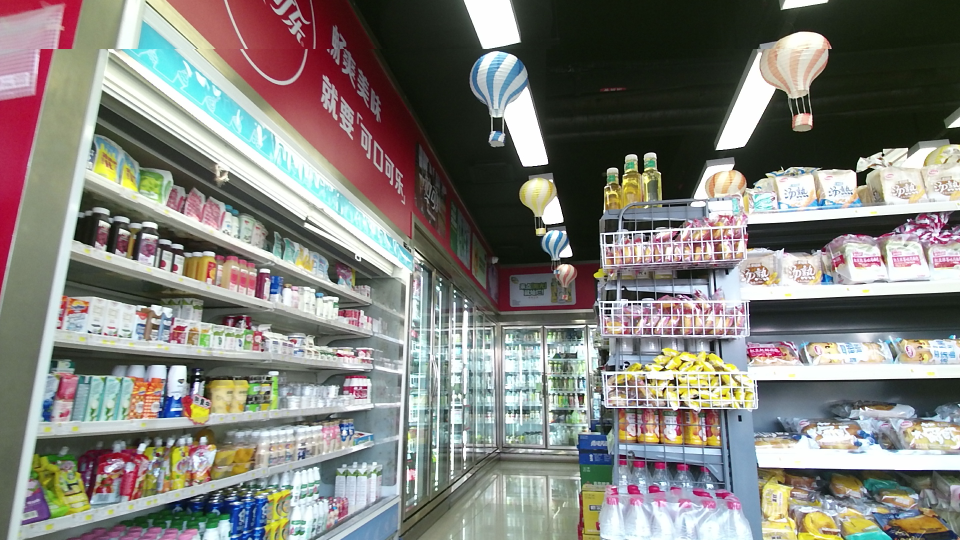
\includegraphics[height=4.1cm,width=.9\linewidth,keepaspectratio]{figures/thud_dense_test50-frame-000007.png}\end{center}\begin{center}\small\begin{tabular}{p{2.2cm}p{1.5cm}p{1.2cm}p{10cm}}\toprule
Model & Detekcija & Regije & Dejanski izsek opisa (model) \\ \midrule
qwen35-bf16 & ok: 5 & ok & A retail aisle view featuring a large refrigerated display unit on the left and multiple shelving units on the right. The ceiling is dark with fluorescent lighting and hanging hot air balloon ... \\
qwen35-q4 & ok: 4 & ok & A retail aisle with refrigerated units on the left and open shelving on the right. Decorative hot air balloon lights hang from the ceiling. The floor is reflective tile. Aisles extend into the... \\
gemma3-q4 & ok: 5 & ok & The photograph depicts a retail environment, likely a supermarket or convenience store. Shelves filled with various products line the walls, extending into the depth of the image. Several refr... \\
\bottomrule\end{tabular}\end{center}
\textbf{Referenčna imena:} Board, Fridge, Lamp, Shelf, Bottle. \textbf{Lastna presoja:} BF16 in Q4 ujameta osnovno razporeditev hladilnega dela levo in polic desno, a združujeta številne instance. Trditev o steklenih vratih levega odprtega hladilnega dela je vprašljiva. Gemma hladilnike postavi na desno ("right side"), kar se ne ujema z glavnim vidnim hladilnim delom levo. To je delni vizualni pregled.
\subsection*{Trgovina / frame-000030}\begin{center}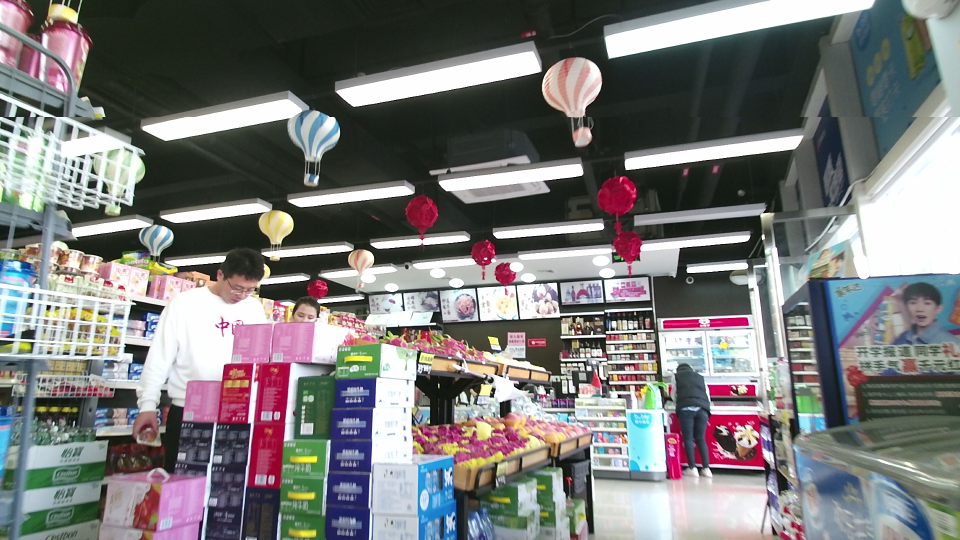
\includegraphics[height=4.1cm,width=.9\linewidth,keepaspectratio]{figures/thud_dense_test50-frame-000030.png}\end{center}\begin{center}\small\begin{tabular}{p{2.2cm}p{1.5cm}p{1.2cm}p{10cm}}\toprule
Model & Detekcija & Regije & Dejanski izsek opisa (model) \\ \midrule
qwen35-bf16 & ok: 8 & ok & An indoor retail environment with stacked product boxes in the foreground and shelving units along walls. Decorative hot air balloon ornaments hang from a black ceiling with fluorescent lighti... \\
qwen35-q4 & ok: 7 & ok & A retail store interior with stacked product boxes in the foreground and shelves along the walls. Decorative hot air balloon ornaments hang from the ceiling alongside rectangular fluorescent l... \\
gemma3-q4 & ok: 6 & ok & The photograph depicts a retail store interior with a focus on a brightly lit section filled with various products. Overhead, several hot air balloon decorations are suspended from the ceiling... \\
\bottomrule\end{tabular}\end{center}
\textbf{Referenčna imena:} Lamp, Shelf, Board, People, Fridge, Freezer, Products, Checkout, Fruits. \textbf{Lastna presoja:} Gost prizor vsebuje zakritost in skupinsko označene izdelke. BF16 izloči moškega v belem ter osebo ob hladilniku; delno zakrite osebe za moškim ne izpostavi. Referenca People ima le dve regiji, zato iz števila okvirjev ne sklepamo o vseh vidnih osebah.

\newpage
\section*{Dejanske slike in primerjava modelov}\subsection*{agtea / frame-000002}\begin{center}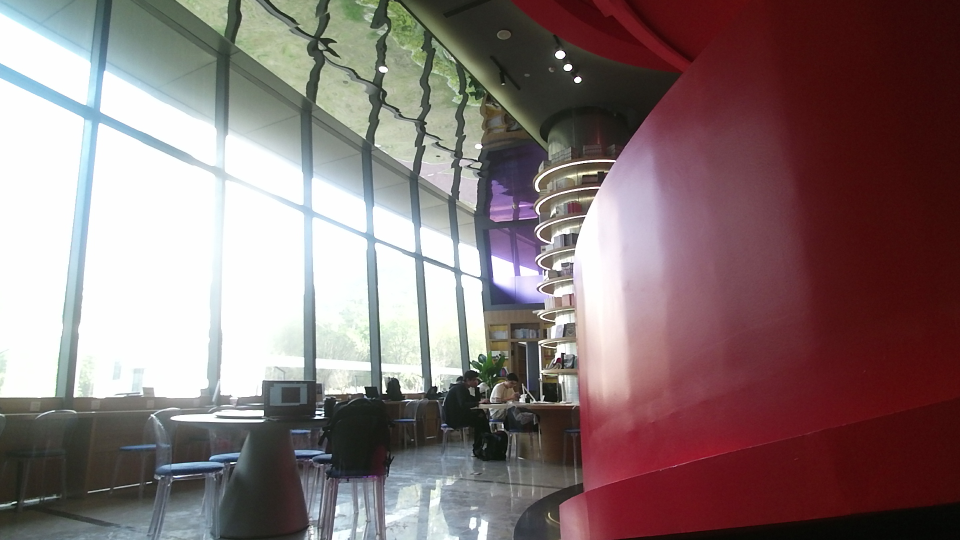
\includegraphics[height=4.1cm,width=.9\linewidth,keepaspectratio]{figures/thud_agtea_test50-frame-000002.png}\end{center}\begin{center}\small\begin{tabular}{p{2.2cm}p{1.5cm}p{1.2cm}p{10cm}}\toprule
Model & Detekcija & Regije & Dejanski izsek opisa (model) \\ \midrule
qwen35-bf16 & ok: 8 & ok & Interior of a modern atrium with large floor-to-ceiling windows on the left allowing bright daylight. A tall, curved red structure dominates the right foreground. In the background, people sit... \\
qwen35-q4 & ok: 4 & ok & An indoor space with large windows on the left allowing bright light. A tall red curved structure dominates the right foreground. In the background, there are tables and chairs, some people se... \\
gemma3-q4 & ok: 5 & error & The photograph depicts a brightly lit interior space, likely a waiting area or lobby. A large window dominates the background, flooding the scene with natural light and revealing a view of tre... \\
\bottomrule\end{tabular}\end{center}
\textbf{Dejanska zavrnitev:} gemma3-q4 / regije: Missing IDs: \{('int', 2)\}
\textbf{Referenčna imena:} People, Chair, Window, Table, Shelf, Bag, Laptop, Plants, Spotlight, Glass, Stairs. \textbf{Lastna presoja:} BF16 stole opiše kot "clear acrylic or plastic"; vidim kovinske cevaste okvirje in modra sedišča, prosojnega materiala ne potrdim. Q4 združi mize in stole v "tables and chairs". Gemma trdi, da je stol na mizi; vidni stoli stojijo na tleh. Njen opis regij izpusti ID 2 in je zavrnjen.
\subsection*{agtea / frame-000026}\begin{center}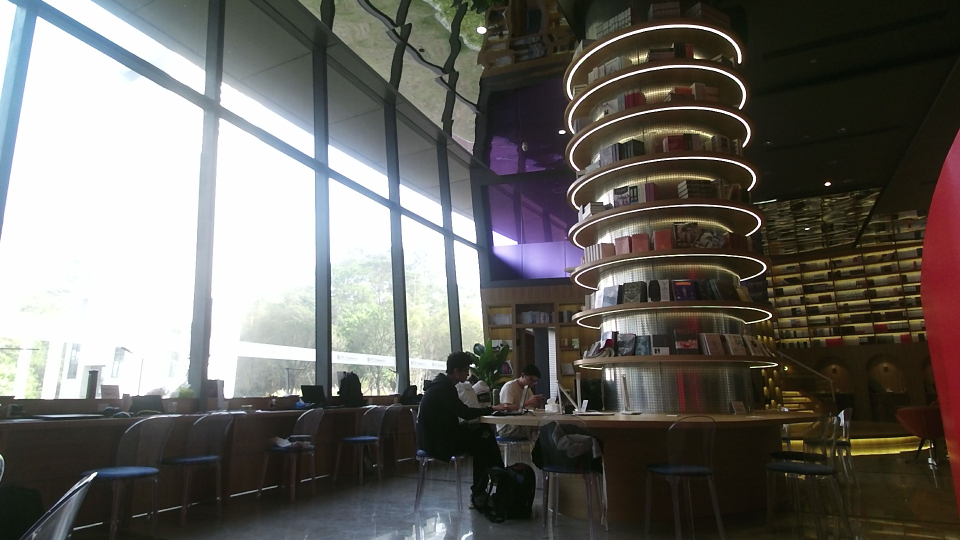
\includegraphics[height=4.1cm,width=.9\linewidth,keepaspectratio]{figures/thud_agtea_test50-frame-000026.png}\end{center}\begin{center}\small\begin{tabular}{p{2.2cm}p{1.5cm}p{1.2cm}p{10cm}}\toprule
Model & Detekcija & Regije & Dejanski izsek opisa (model) \\ \midrule
qwen35-bf16 & ok: 5 & ok & An indoor public space with large windows on the left and a spiral bookshelf structure in the center. People are seated at tables near the window. The floor is reflective. A red curved object ... \\
qwen35-q4 & ok: 6 & error & An indoor public space with large windows on the left and a spiral bookshelf structure in the center. Several people are seated at tables near the window, working or reading. The room has mode... \\
gemma3-q4 & ok: 5 & ok & The photograph depicts a brightly lit interior space, likely a library or bookstore, with a large, circular bookshelf dominating the central view. The bookshelf is illuminated from within and ... \\
\bottomrule\end{tabular}\end{center}
\textbf{Dejanska zavrnitev:} qwen35-q4 / regije: A supplied label was changed.
\textbf{Referenčna imena:} People, Chair, Window, Table, Shelf, Stairs, Bag, Laptop, Glass, Plants, Book. \textbf{Lastna presoja:} Vidna sta osvetljena krožna knjižna polica in več stolov; osebe, knjige in torbe so delno zakrite. Lokacija ob steni ali veliki konstrukciji sama po sebi ne dokazuje trajne stabilnosti. Celoten ročni pregled vseh instanc še ni opravljen.

\newpage
\section*{Utemeljitve, napake in omejitve}
Naslednji izseki so besedni razlogi modela; niso lastna potrditev vidnih dokazov. Primeri so izbrani iz vrat, slik, polic in pohištva, kjer so te vrste dejansko vrnjene. Hladilnih vrat ne enačimo z vrati prostora. Če slik/umetniških del opisovalnik ne izloči, njihovega razvrščanja ne prikazujemo kot izmerjenega. Celotni pari z imenom poskusa in SHA256 so v \texttt{reasoning-comparisons.csv}.
\begin{center}\small\begin{tabular}{p{3.3cm}p{3.1cm}p{8.7cm}}\toprule
Objekt & Osnova $\rightarrow$ različica & Dejanski modelov razlog \\ \midrule
Vrata: Glass door & fixed $\rightarrow$ fixed & Structural building element; opening is not relocation.\newline{\scriptsize trgovina / image-000050 / ID 2 / long-examples-t0.3-s42} \\
Slike & -- & Ni samostojnega predmeta te vrste v primerjanih veljavnih opisih. \\
Police: shelving unit & fixed $\rightarrow$ uncertain & Shelving could be bolted or on wheels; evidence missing.\newline{\scriptsize trgovina / image-000006 / ID 5 / long-examples-t0.3-s42} \\
Pohištvo: desk & movable $\rightarrow$ fixed & Desk is a structural element integrated into the room layout.\newline{\scriptsize agtea / image-000012 / ID 2 / long-no-examples-t0-s42} \\
\bottomrule\end{tabular}\end{center}

V besedilnem delu je 5 odgovorov brez obvezne utemeljitve in 2 s podvojenim ključem ter 1 z drugimi kršitvami sheme. Vsi ostanejo zavrnjeni s shranjenim surovim odgovorom; podvojenega ključa ne razrešimo z izbiro zadnje vrednosti.
\subsection*{NVILA 8B}
Dodatni model ni izveden. Omejena začetna diagnostika: uradna validacijska shema ne vključuje \texttt{NVILA-8B}, izolirani venv pa je odpovedal zaradi manjkajočega ensurepip. Uteži niso prenesene in slikovni API ni preverjen; 8B ni preimenovan v 15B. Celotne ovire in viri so v \texttt{nvila-diagnostic.json}.
\subsection*{Ponovljivost in izvor}
Preverjanje kode: 54 testov (OK); revizija 34/34 skupin, 0 kršitev nespremenljivih vhodov/GPU. Podrobnosti: tests.json in verification.json. Izhodiščni Git commit: \texttt{399d6ea6c53f}. Različice, gonilnik in slika Docker so v \texttt{environment.json}; točna natančnost, slikovni projektor in zmožnosti v manifestih posameznih poskusov. Konfiguracije vsebujejo vse nastavitve, shranjeni odgovori pa prompte, SHA256 slike/opisa, čas, možnosti, GPU stanje in surovi API odgovor.
\begin{verbatim}
bash scripts/thud_experiment.sh --phase all
python3 -m llm_object_classifier.thud_q4_repeat
python3 -m llm_object_classifier.thud_verify --require-complete
python3 -m llm_object_classifier.thud_report
bash scripts/compile_thud_report.sh
python3 -m unittest discover -s tests -v
\end{verbatim}
Zaganjalnik uporablja projektno Ollamo (privzeti omrežni naslov lahko nastavimo z \texttt{--base-url}). Predpogoji: zdrava GPU Ollama, preneseni trije tagi, Python s Pillow. Vsaka dokončana skupina dobi oznako; nadaljevanje preverja nespremenljivost vhodov in ne prepisuje odgovorov. Prekinjeni poskusi drugega koraka ostanejo kot ločeni poskusi.
Veliki surovi izhodi: \texttt{results/thud-vmesno/}. Majhen paket PDF/LaTeX, slike, agregati, izbor, preglednica in metodologija: \texttt{reports/THUD\_VMESNO/}. Stari NYU poskusi ostanejo ločeni.
\subsection*{Naslednji utemeljeni poskus}
Za naslednji ročni pregled izberemo kratki prompt brez primerov kot kandidata: primerjava sheme zgoraj podpira njegov operativni preizkus, ne dokazuje pravilnosti. Preveriti je treba iste objekte in razhajanja proti dolgemu promptu s primeri, predvsem pri policah in pohištvu. Hitrost ponoviti ob izključni uporabi GPU. Šele po primerljivi ročno potrjeni kakovosti izbrati končni prompt. To je sklep 1. dela: predlog nadaljevanja so bogatejši odnosi in vidni dokazi; dejanski 2. del je po izrecnem naročilu dokumentiran v nadaljevanju tega poročila, kadar je dodatek prisoten. NVILA ostaja ločena priprava.
\vfill{\footnotesize Uradni viri: \href{https://ollama.com/library/qwen3.5:4b-bf16}{Qwen BF16}, \href{https://ollama.com/library/qwen3.5:4b-q4_K_M}{Qwen Q4}, \href{https://ollama.com/library/gemma3:4b-it-q4_K_M}{Gemma Q4}, \href{https://huggingface.co/Efficient-Large-Model/NVILA-8B}{NVILA uteži}, \href{https://github.com/NVlabs/VILA/blob/main/server.py}{NVILA strežnik}. Preverjeno 20. 10. 2026.}

\newpage
\section*{2. del: bogatejši samostojni opis (21. 10. 2026)}
Nadaljevanje uporablja obstoječe izhode 1. dela (objavljen commit \texttt{7509607}); uspešni stari klici se ne ponovijo. Vsi trije delujoči modeli prejmejo iste slikovne bajte vseh 100 slik, brez referenčnih imen, ID, okvirjev ali poti anotacij. NVILA še nima preverjenega slikovnega API; njegova že shranjena diagnostika se uporabi brez novega prenosa ali trditve o inferenci.
\subsection*{Izhodna shema in dokazi}
\texttt{rich-description-v2} ohrani \texttt{scene\_description} in stare združljive podatke objektov, doda \texttt{appearance}, \texttt{image\_location}, \texttt{occlusion}, \texttt{support\_contacts}, \texttt{installation\_evidence} ter seznam \texttt{relations}. Odnos navaja začetni/ciljni lokalni ID, predikat in vidni dokaz. Validator zavrne manjkajoče podatke, podvojene ID/odnose, sklice na neobstoječe ID, samopovezave in razrede stabilnosti v prvem koraku. Neznano je izrecno \texttt{unknown}. Nobeno besedilno polje samo ne dokazuje pravilnosti trditve.
Položaji opisujejo levo/desno v sliki, ne svetovnih koordinat. Skritih vijakov, teže ali trajnosti ne zahtevamo; bližina ali negibnost ni namestitev. ID so lokalni, brez sledenja skozi čas. Napovedanih okvirjev ni; besedni položaj ni meritev natančne lokalizacije. Zato ni IoU ali mAP in na teh rezultatih še ni podlage za uvedbo posebnega detektorja.
\subsection*{Primerjava časa in oblike izhoda}
\begin{center}\small\begin{tabular}{llrrrrrrr}\toprule
Opisovalnik & Različica & OK/vsi & Med. & p90 & Povp. & Tok. & tok/s & GiB \\ \midrule
qwen35-bf16 & 1. del, podrobni & 100/100 & 4.5 & 15.4 & 7.2 & 510 & 73.3 & 8.78 \\
qwen35-bf16 & 2. del, bogati & 69/100 & 11.5 & 19.0 & 13.3 & 1130 & 87.7 & 8.78 \\
qwen35-q4 & 1. del, podrobni & 100/100 & 2.7 & 4.8 & 3.1 & 521 & 180.7 & 3.40 \\
qwen35-q4 & 2. del, bogati & 82/100 & 4.1 & 6.1 & 5.1 & 1116 & 232.7 & 3.40 \\
gemma3-q4 & 1. del, podrobni & 100/100 & 3.1 & 6.2 & 3.7 & 593 & 176.7 & 2.85 \\
gemma3-q4 & 2. del, bogati & 89/100 & 4.2 & 5.3 & 4.2 & 857 & 225.6 & 2.85 \\
\bottomrule\end{tabular}\end{center}

Časi so sekunde na sliko, tudi za zavrnjene odgovore z izmerjenim časom. Tok. je povprečje izhodnih tokenov, tok/s pa hitrost API generiranja. GiB je največja API dodelitev VRAM. Ogrevanje in nalaganje sta ločena v \texttt{part2-aggregates.json}. GPU je deljen; obremenitev in dolžina odgovora omejujeta vzročno primerjavo hitrosti. Stari prompt je podroben, novi je drugačen prompt s strožjo shemo; razlike ne pripisujemo samo strukturiranju.
Prekopirano pilotno ogrevanje ne pomeni ogretega modela po novem nalaganju. Prvi novi klic (indeks 3) posamezne skupine lahko vključuje nalaganje; celotni čas ostane v tabeli, API \texttt{load\_duration} je ohranjen ločeno. To je dodatna omejitev neposredne primerjave hitrosti, ne prikrita izločitev počasnih klicev.
\begin{center}\small\begin{tabular}{lrrrrr}\toprule
Model & Objekti & Odnosi & Opisi z odnosi & Namest. unknown & Podpora unknown \\ \midrule
qwen35-bf16 & 473 & 182 & 61/69 & 437 & 468 \\
qwen35-q4 & 539 & 218 & 82/82 & 513 & 539 \\
gemma3-q4 & 525 & 151 & 74/89 & 330 & 523 \\
\bottomrule\end{tabular}\end{center}

Objekti in odnosi so šteti le v sprejetih opisih; zavrnitve ostanejo v imenovalcih zgornje tabele. Število odnosov/objektov in prisotnost polj merita strukturo, ne pravilnosti, priklica ali vidnih dokazov. Neznano šteje le dobesedni \texttt{unknown}, ne vseh izrazov negotovosti. Vsi sprejeti odnosi imajo veljavne sklice in neprazno besedilo dokaza; ta pogoj ne potrdi vsebine fotografije.

Predhodna diagnostika prvega prompta: 1/12 po shemi, 6 ločenih ogrevanj. Zaradi izpuščenih tipov je dodana izrecna JSON tipovna predloga brez vsebinskih primerov; validator in generacijske nastavitve niso razrahljani. Diagnostični odgovori so ohranjeni ločeno in niso prišteti končni primerjavi; ne gre za prikrito popravljanje izhodov.

\newpage
\section*{2. del: vpliv opisov na besedilno presojo}
Isti izbor 10+10 slik ostane zamrznjen. Razvrščevalnik Qwen BF16 dobi celoten shranjeni opis, strukturirane objekte in odnose, brez odpiranja fotografije. Uporabljen je isti kratki prompt brez primerov iz 1. dela pri T=.3, seed 42; izbran je zaradi uspešne izpolnitve sheme, ne potrjene vsebinske prednosti. Stare BF16 odločitve se uporabijo ponovno, manjkajoče kontrole starih Q4/Gemma opisov se izvedejo le enkrat.
\begin{center}\small\begin{tabular}{llrrrrrr}\toprule
Opisovalnik & Vhod & OK/vsi & Preskoki & F & M & U & Med. [s] \\ \midrule
qwen35-bf16 & stari opis & 20/20 & 0 & 37 & 63 & 15 & 1.6 \\
qwen35-bf16 & bogati opis & 10/20 & 7 & 22 & 33 & 9 & 1.2 \\
qwen35-q4 & stari opis & 15/20 & 0 & 25 & 48 & 14 & 1.0 \\
qwen35-q4 & bogati opis & 15/20 & 4 & 24 & 63 & 22 & 1.4 \\
gemma3-q4 & stari opis & 18/20 & 0 & 26 & 63 & 9 & 1.0 \\
gemma3-q4 & bogati opis & 16/20 & 1 & 33 & 51 & 12 & 1.2 \\
\bottomrule\end{tabular}\end{center}

F/M/U so števila odločitev v sprejetih odgovorih. Preskok pomeni zavrnjen vhodni opis; ostane v imenovalcu vseh 20 položajev. Drugačno število objektov med starimi in novimi opisi pomeni, da skupnih ID ne moremo obravnavati kot iste instance.
\begin{center}\small\begin{tabular}{lrr}\toprule
Opisovalnik & Pari imen & Spremembe razreda \\ \midrule
qwen35-bf16 & 13 & 3 \\
qwen35-q4 & 16 & 5 \\
gemma3-q4 & 28 & 6 \\
\bottomrule\end{tabular}\end{center}

Pari so le enolična, natančno enaka imena po pretvorbi v male črke in normalizaciji presledkov v obeh veljavnih izhodih iste slike. Podvojena imena se izključijo; sinonimov in okvirjev ne ujemamo. To ni potrjeno ujemanje instanc; skupinska imena so posebej problematična. Sprememba ali strinjanje ni pravilnost. Konkretni pari, ID, SHA256 obeh opisov in oba modelova razloga so v \texttt{part2-decision-pairs.csv}.
\subsection*{Ožja kontrola prompta BF16 na istih 20 slikah}
\begin{center}\small\begin{tabular}{lrrr}\toprule
Različica opisa BF16 & OK/vsi & Med. [s] & Objekti \\ \midrule
1. del kratek & 20/20 & 3.4 & 81 \\
2. del bogati & 13/20 & 12.2 & 80 \\
\bottomrule\end{tabular}\end{center}

Oba prompta sta brez vsebinskih primerov in pri T=0, seed 42. Kratki stari opis se ponovno uporabi iz 1. dela. Nova shema in besedilo se še vedno spreminjata skupaj, zato to ni izolirana ablacija sheme. Za Q4/Gemma primerljivega starega kratkega opisa ni; dodatnih starih klicev za to ne izvajamo.
\subsection*{Obseg, revizija in ponovljivost}
Položajev glavne primerjave: 400; odgovorov 388; preskokov 12. Pilot: 12 odgovorov, od tega 12 prekopiranih v glavno primerjavo, brez ponovnega klica. Enkratnih novih merjenih odgovorov brez prve diagnostike: 388. Ločena nova ogrevanja: 16; 6 njihovih kopij se ne šteje ponovno. Revizija 24/24 skupin, kršitev 0; nespremenjenih starih odgovorov 846. Testi: 61 (OK).
End-to-end čas novih faz brez predhodne diagnostike: 41.7 min; pilotne kopije in 20 starih presoj niso šteti ponovno. Nalaganje in ogrevanje sta podrobno ločena v agregatih; warmup\_reused\_from\_pilot označi kopijo ogrevanja, new\_warmup\_calls pa dejanske nove klice. Za prihodnje sveže zagone je kopiranje ogrevanja odpravljeno; izvirne meritve in njihov nalagalni strošek ostanejo nespremenjeni.
\begin{verbatim}
bash scripts/thud_part2.sh --phase all
python3 -m llm_object_classifier.thud_part2_report --require-complete
python3 -m llm_object_classifier.thud_report
bash scripts/compile_thud_report.sh
\end{verbatim}
Surovi izhodi: \texttt{results/thud-part2/}; izvorni 1. del ostane v \texttt{results/thud-vmesno/}. Dopolnjeni pregled s fotografijami, referenčnimi okvirji, vsemi strukturami in odločitvami: \texttt{results/thud-part2/manual-review.html}. Konfiguracije, SHA256 kode, stanje Gita in modeli so v lokalnih manifestih/snapshotih. Ponovni zagon ohrani tudi zavrnitve in preskoke; spremenjeni vhodi se zavrnejo.

\newpage
\section*{2. del: dejanski primeri bogatejšega opisa}\subsection*{thud\_dense\_test50/frame-000007}\begin{center}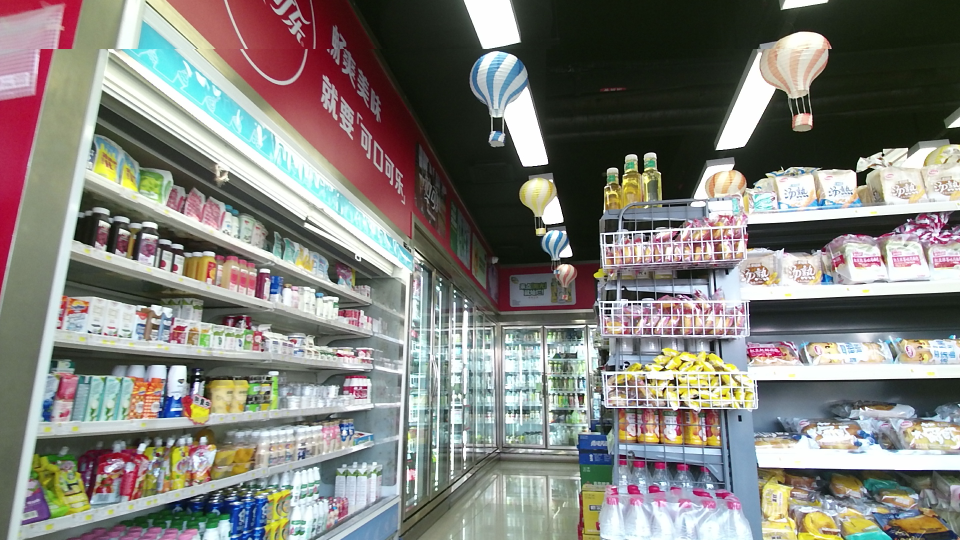
\includegraphics[height=3.2cm,width=.8\linewidth,keepaspectratio]{figures/thud_dense_test50-frame-000007.png}\end{center}\begin{center}\small\begin{tabular}{p{2.2cm}p{2.1cm}p{10.7cm}}\toprule
Model & Obj./odnosi & Dejanski prvi modelov odnos ali napaka \\ \midrule
qwen35-bf16 & zavrnjeno & Unknown relation predicate. \\
qwen35-q4 & 8/3 & refrigerated display unit beside metal shelving unit: separated by an aisle floor \\
gemma3-q4 & 5/2 & hot air balloon beside shelving unit: The hot air balloon is positioned beside the shelving unit. \\
\bottomrule\end{tabular}\end{center}
\textbf{Lastna presoja:} Q4 in Gemma pravilno postavita glavni hladilni del levo, police desno; Gemma je v starem opisu hladilnike postavila desno. Gemmina nova trditev o lesenih policah ni podprta: vidni nosilci so kovinski. Q4 navaja visible\_installation, hkrati installation\_evidence=unknown; samega vidnega znaka ne štejemo za dokaz pritrditve celotnega hladilnika. BF16 je zavrnjen zaradi above/below zunaj slovarja, ne zaradi samega prostorskega pomena. Vsi trije še združujejo izdelke. To je delni vizualni pregled.
\subsection*{thud\_dense\_test50/frame-000030}\begin{center}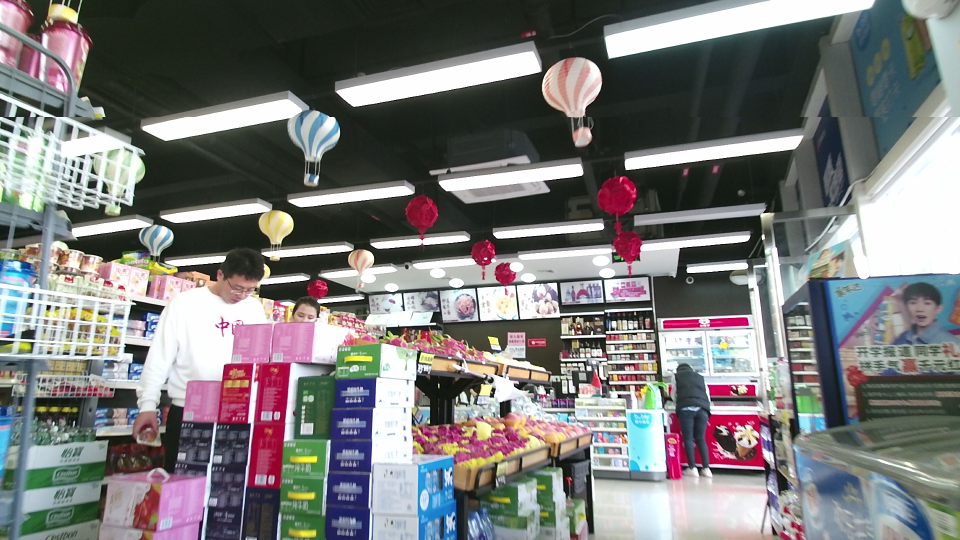
\includegraphics[height=3.2cm,width=.8\linewidth,keepaspectratio]{figures/thud_dense_test50-frame-000030.png}\end{center}\begin{center}\small\begin{tabular}{p{2.2cm}p{2.1cm}p{10.7cm}}\toprule
Model & Obj./odnosi & Dejanski prvi modelov odnos ali napaka \\ \midrule
qwen35-bf16 & 10/4 & person beside stacked boxes: standing next to stacked boxes \\
qwen35-q4 & 10/2 & person beside beverage boxes: Person stands next to stacked beverage boxes. \\
gemma3-q4 & zavrnjeno & Unknown relation predicate. \\
\bottomrule\end{tabular}\end{center}
\textbf{Lastna presoja:} BF16 zdaj loči tri osebe; delno zakrito osebo za moškim označi partial in poveže z behind, stari osnovni opis je ni izpostavil. Q4 in Gemmin zavrnjeni kandidat še navedeta le dve osebi. Referenca People ima le dve regiji, zato tega ne pretvorimo v samodejni priklic. Q4-jev razlog near the refrigerator ne podpira predikata behind. Gemmin kandidat je zavrnjen zaradi above; hkrati opis partially obscured združi z occlusion=none. Trditve BF16 o hoji iz ene fotografije ne morem potrditi. Podpore ostanejo unknown. Delni vizualni pregled, tudi zavrnjenega kandidata.
\subsection*{Dejanski besedni razlogi pri parih imen}\begin{center}\small\begin{tabular}{p{5.6cm}p{2.8cm}p{6.5cm}}\toprule
Opisovalnik / slika / ime & Staro -> bogato & Razlog modela na bogatem opisu \\ \midrule
qwen35-bf16 / agtea / image-000045 / large windows & fixed -> uncertain & Windows fixed to building but evidence is not visible. \\
qwen35-q4 / trgovina / image-000012 / refrigerated display case & uncertain -> movable & Refrigerated display case typically freestanding in retail. \\
gemma3-q4 / trgovina / image-000028 / person & movable -> uncertain & Person status varies; walking implies temporary presence. \\
\bottomrule\end{tabular}\end{center}
To so modelove utemeljitve, ne potrjena referenca; ujemanje imena ne potrdi iste instance.

\newpage
\section*{2. del: dejanski primeri bogatejšega opisa}\subsection*{thud\_agtea\_test50/frame-000002}\begin{center}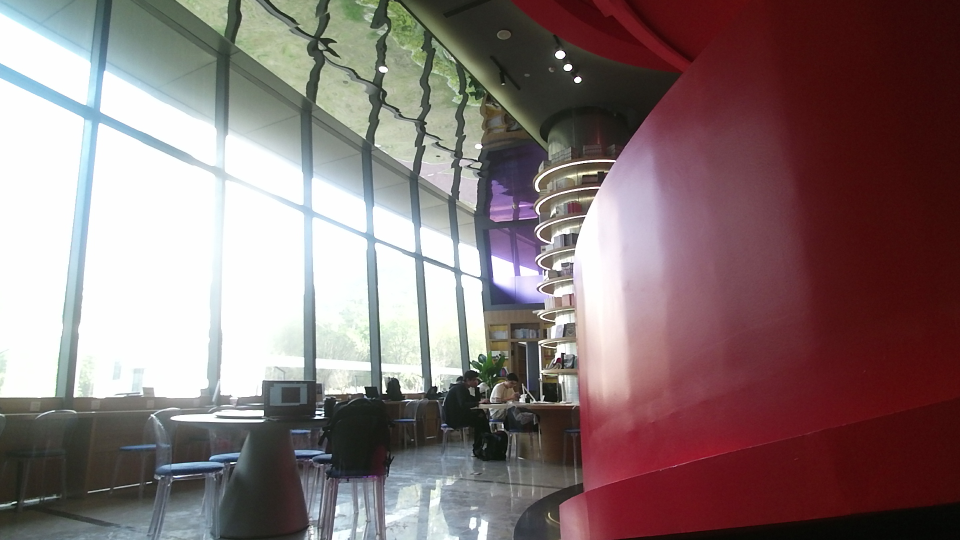
\includegraphics[height=3.2cm,width=.8\linewidth,keepaspectratio]{figures/thud_agtea_test50-frame-000002.png}\end{center}\begin{center}\small\begin{tabular}{p{2.2cm}p{2.1cm}p{10.7cm}}\toprule
Model & Obj./odnosi & Dejanski prvi modelov odnos ali napaka \\ \midrule
qwen35-bf16 & 5/0 & Brez odnosov. \\
qwen35-q4 & 5/2 & red curved structure beside spiral shelving unit: red structure is adjacent to shelving unit \\
gemma3-q4 & 6/3 & Table beside Chair: The table and chair are positioned adjacent to each other. \\
\bottomrule\end{tabular}\end{center}
\textbf{Lastna presoja:} BF16 tudi v novem veljavnem izhodu stole opiše kot transparent plastic; vidim kovinske cevne okvirje in modra sedišča. Q4 še združuje tables and chairs. Gemma okno postavi right/top/full, čeprav prevladuje na levi; vijolične svetilke, ki jo navede, ne morem potrditi. BF16 ne vrne nobenega odnosa; Q4 in Gemma vrneta odnose, vendar to še ne potrdi njihove vsebine. Pri vidnih stolih in mizah ostanejo podpore unknown. To je delni vizualni pregled, ne popolna referenca stabilnosti.
\subsection*{thud\_agtea\_test50/frame-000026}\begin{center}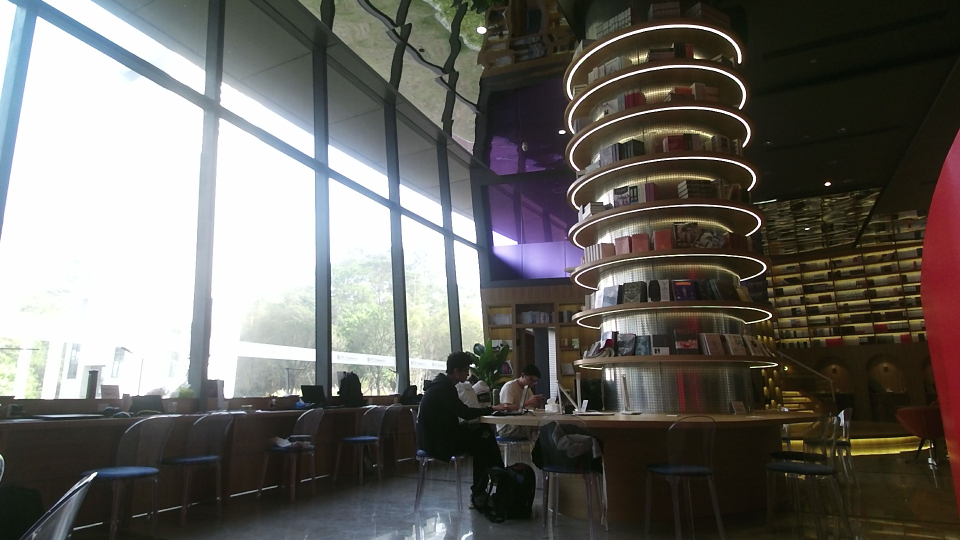
\includegraphics[height=3.2cm,width=.8\linewidth,keepaspectratio]{figures/thud_agtea_test50-frame-000026.png}\end{center}\begin{center}\small\begin{tabular}{p{2.2cm}p{2.1cm}p{10.7cm}}\toprule
Model & Obj./odnosi & Dejanski prvi modelov odnos ali napaka \\ \midrule
qwen35-bf16 & zavrnjeno & Unknown relation predicate. \\
qwen35-q4 & 8/3 & person beside person: seated next to each other at the table \\
gemma3-q4 & 6/3 & Circular Bookshelf beside Chair: The circular bookshelf is beside the chair. \\
\bottomrule\end{tabular}\end{center}
\textbf{Lastna presoja:} BF16 kandidat je zavrnjen zaradi at in near; zato ne gre v razvrščanje. Dve osebi, krožna polica in modri kovinski stoli v njem so vizualno smiselni, a zakritost vseh označi none. Q4 sprejeti opis loči dve osebi in stola z modrim sediščem; odnos miza under spiral bookshelf zahteva presojo stika in globine, ne le vertikalnega položaja. Gemma si izmisli sive pisarniške stole z nasloni za roke in drugo osebo postavi desno, čeprav sta vidni osebi levo od krožne police. Vsi ohranijo podpore unknown. Namestitve police ne morem potrditi. Delni vizualni pregled, tudi zavrnjenega kandidata.
\subsection*{Sklep in naslednji poskus}Bogatejši zapis omogoča pregled zakritosti in odnosov ter konkreten popravek pri tretji osebi v gostem prizoru. Ne potrjuje pa splošne izboljšave: sprejeti JSON še vsebuje napačne materiale, lokacije in nepodprte dokaze namestitve, številne podpore ostanejo neznane. Večja shema poveča izhod in prinese dodatne zavrnitve. Naslednji kontrolirani poskus naj na istih 20 slikah najprej razjasni slovar odnosov ob nespremenjenih drugih pogojih, nato ločeno preveri tipovno predlogo brez privzetih vrednosti unknown. Neznano mora ostati dovoljeno, kadar dokaz ni viden. Pred končno izbiro modela/prompta je potreben sistematičen ročni pregled istih objektov in stikov. Največ veljavnih JSON ni dokaz najboljše vsebine; brez referenc stabilnosti accuracy ostaja nedoločena.

\end{document}
